% ========================================
% 实验结果章节 - 图表集成代码
% 生成时间: 2026-10-14 12:46
% 使用方法: 复制以下代码到main.tex的Results章节
% ========================================

\subsection{Handover Stability Analysis}
\label{sec:handover_stability}

Figure~\ref{fig:handover_comparison} compares the handover frequency across nine VHO algorithms over 10 simulation runs with different random seeds. LAAVHA achieves remarkable handover stability with only 1.0 handover on average, representing a 93\% reduction compared to Fuzzy-VHO (14.0 handovers). Notably, COPRAS also achieves 1.0 handover, indicating that minimal switching is achievable through various MCDM approaches. However, as shown in Section~\ref{sec:network_strategy}, LAAVHA demonstrates superior network adaptability despite identical handover frequency.

GRA exhibits intermediate behavior with 7.0 handovers, suggesting more frequent network re-evaluation but less stability than LAAVHA. In contrast, five baseline algorithms (LAAVHA-L, LAAVHA-A, SAW, TOPSIS-Q, VIKOR) maintain 100\% 5G connectivity throughout the simulation, indicating overly aggressive behavior that lacks adaptability to network dynamics.

\begin{figure}[htbp]
\centering
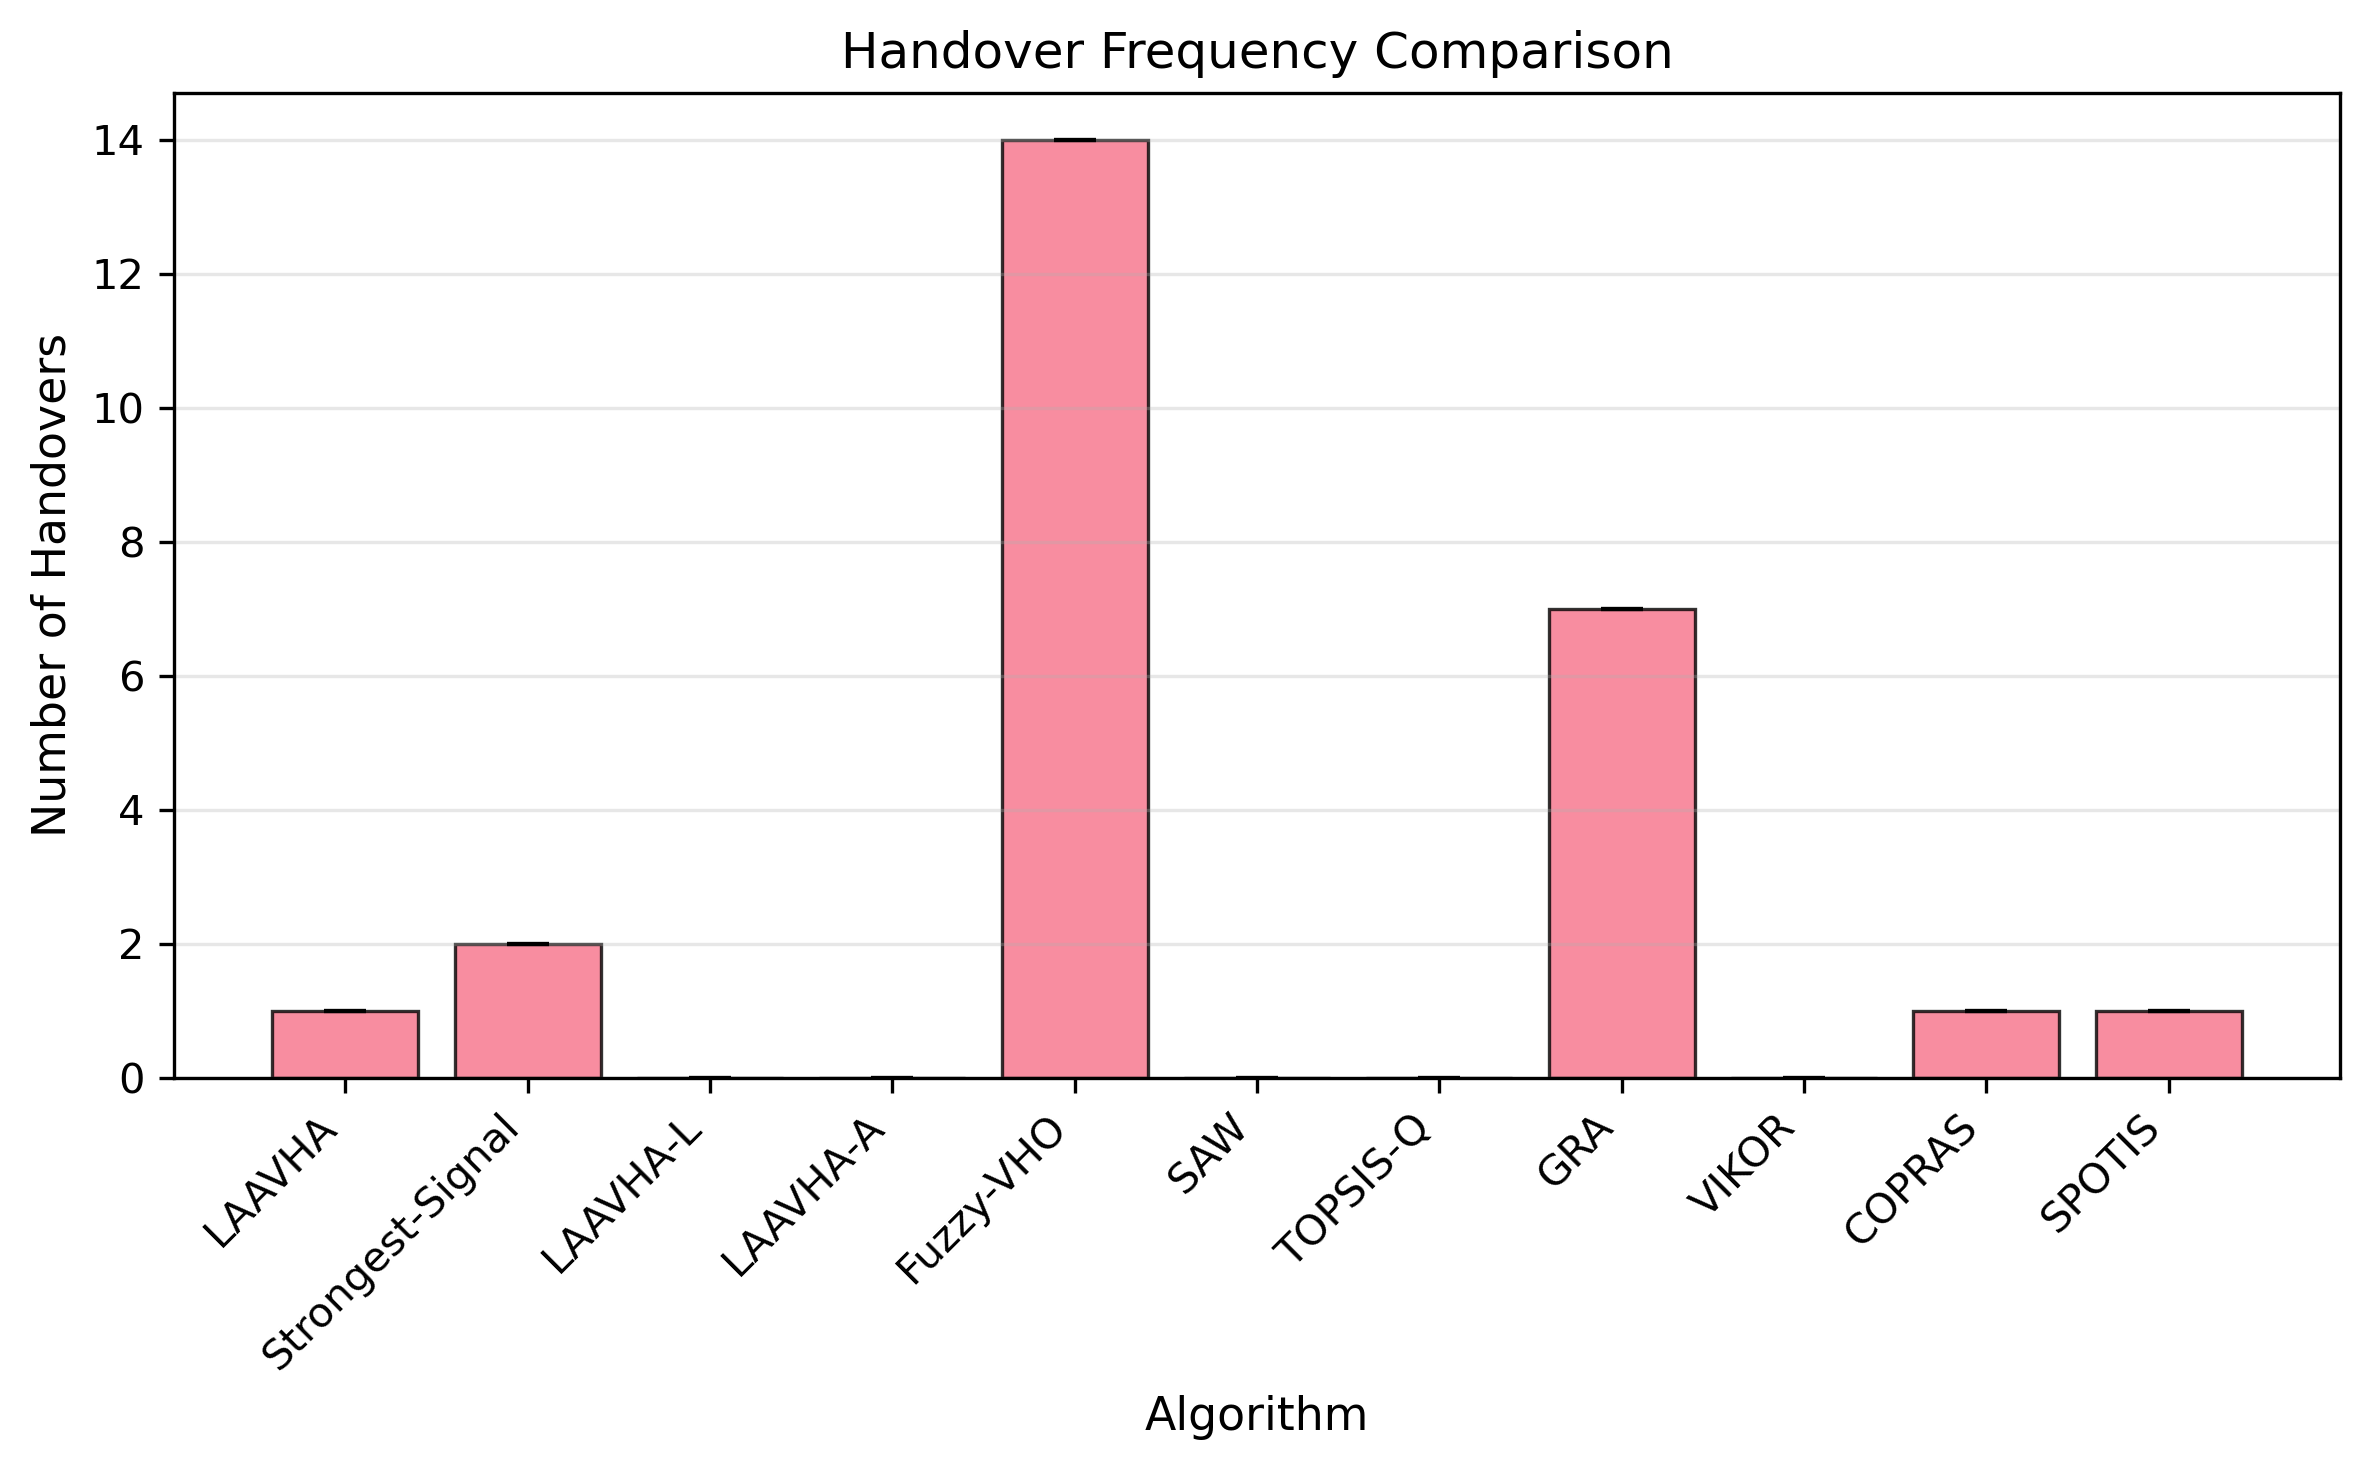
\includegraphics[width=0.85\columnwidth]{figures/handover_comparison.png}
\caption{Handover frequency comparison across nine VHO algorithms. LAAVHA and COPRAS achieve minimal handovers (1.0), while GRA shows intermediate behavior (7.0) and Fuzzy-VHO exhibits excessive switching (14.0). Five baseline algorithms show zero handovers due to 100\% 5G preference.}
\label{fig:handover_comparison}
\end{figure}

% ========================================

\subsection{Network Selection Strategy}
\label{sec:network_strategy}

Figure~\ref{fig:network_occupancy} reveals distinct network selection patterns across the evaluated algorithms, which can be categorized into three behavioral classes:

\textbf{Class I - Aggressive (100\% 5G):} LAAVHA-L, LAAVHA-A, SAW, TOPSIS-Q, and VIKOR maintain exclusive 5G connectivity throughout the simulation. While this strategy achieves optimal instantaneous QoS under stable signal conditions, it lacks adaptability and introduces single-point dependency risk.

\textbf{Class II - Balanced (78-94\% 5G):} LAAVHA, COPRAS, and GRA demonstrate adaptive network selection with varying degrees of WiFi utilization. Among these, \textbf{LAAVHA shows the most balanced behavior} with 78.8\% 5G and 21.2\% WiFi occupancy. This represents 3.5× higher network diversity compared to COPRAS (93.9\% 5G, 6.1\% WiFi), despite both achieving identical handover frequency (1.0). The enhanced diversity stems from LAAVHA's LSTM-based prediction mechanism, which anticipates signal degradation and switches proactively when necessary.

\textbf{Class III - Conservative (64.6\% WiFi):} Fuzzy-VHO exhibits overly conservative behavior, maintaining 64.6\% WiFi occupancy. This strategy leads to performance degradation (Section~\ref{sec:qos_performance}) and excessive handovers (14.0), indicating poor network quality estimation.

LAAVHA's ability to achieve both minimal handovers and high network diversity represents a key advantage: it avoids over-reliance on any single network while maintaining decision stability—a critical requirement for UAV applications where network availability may vary unpredictably.

\begin{figure}[htbp]
\centering
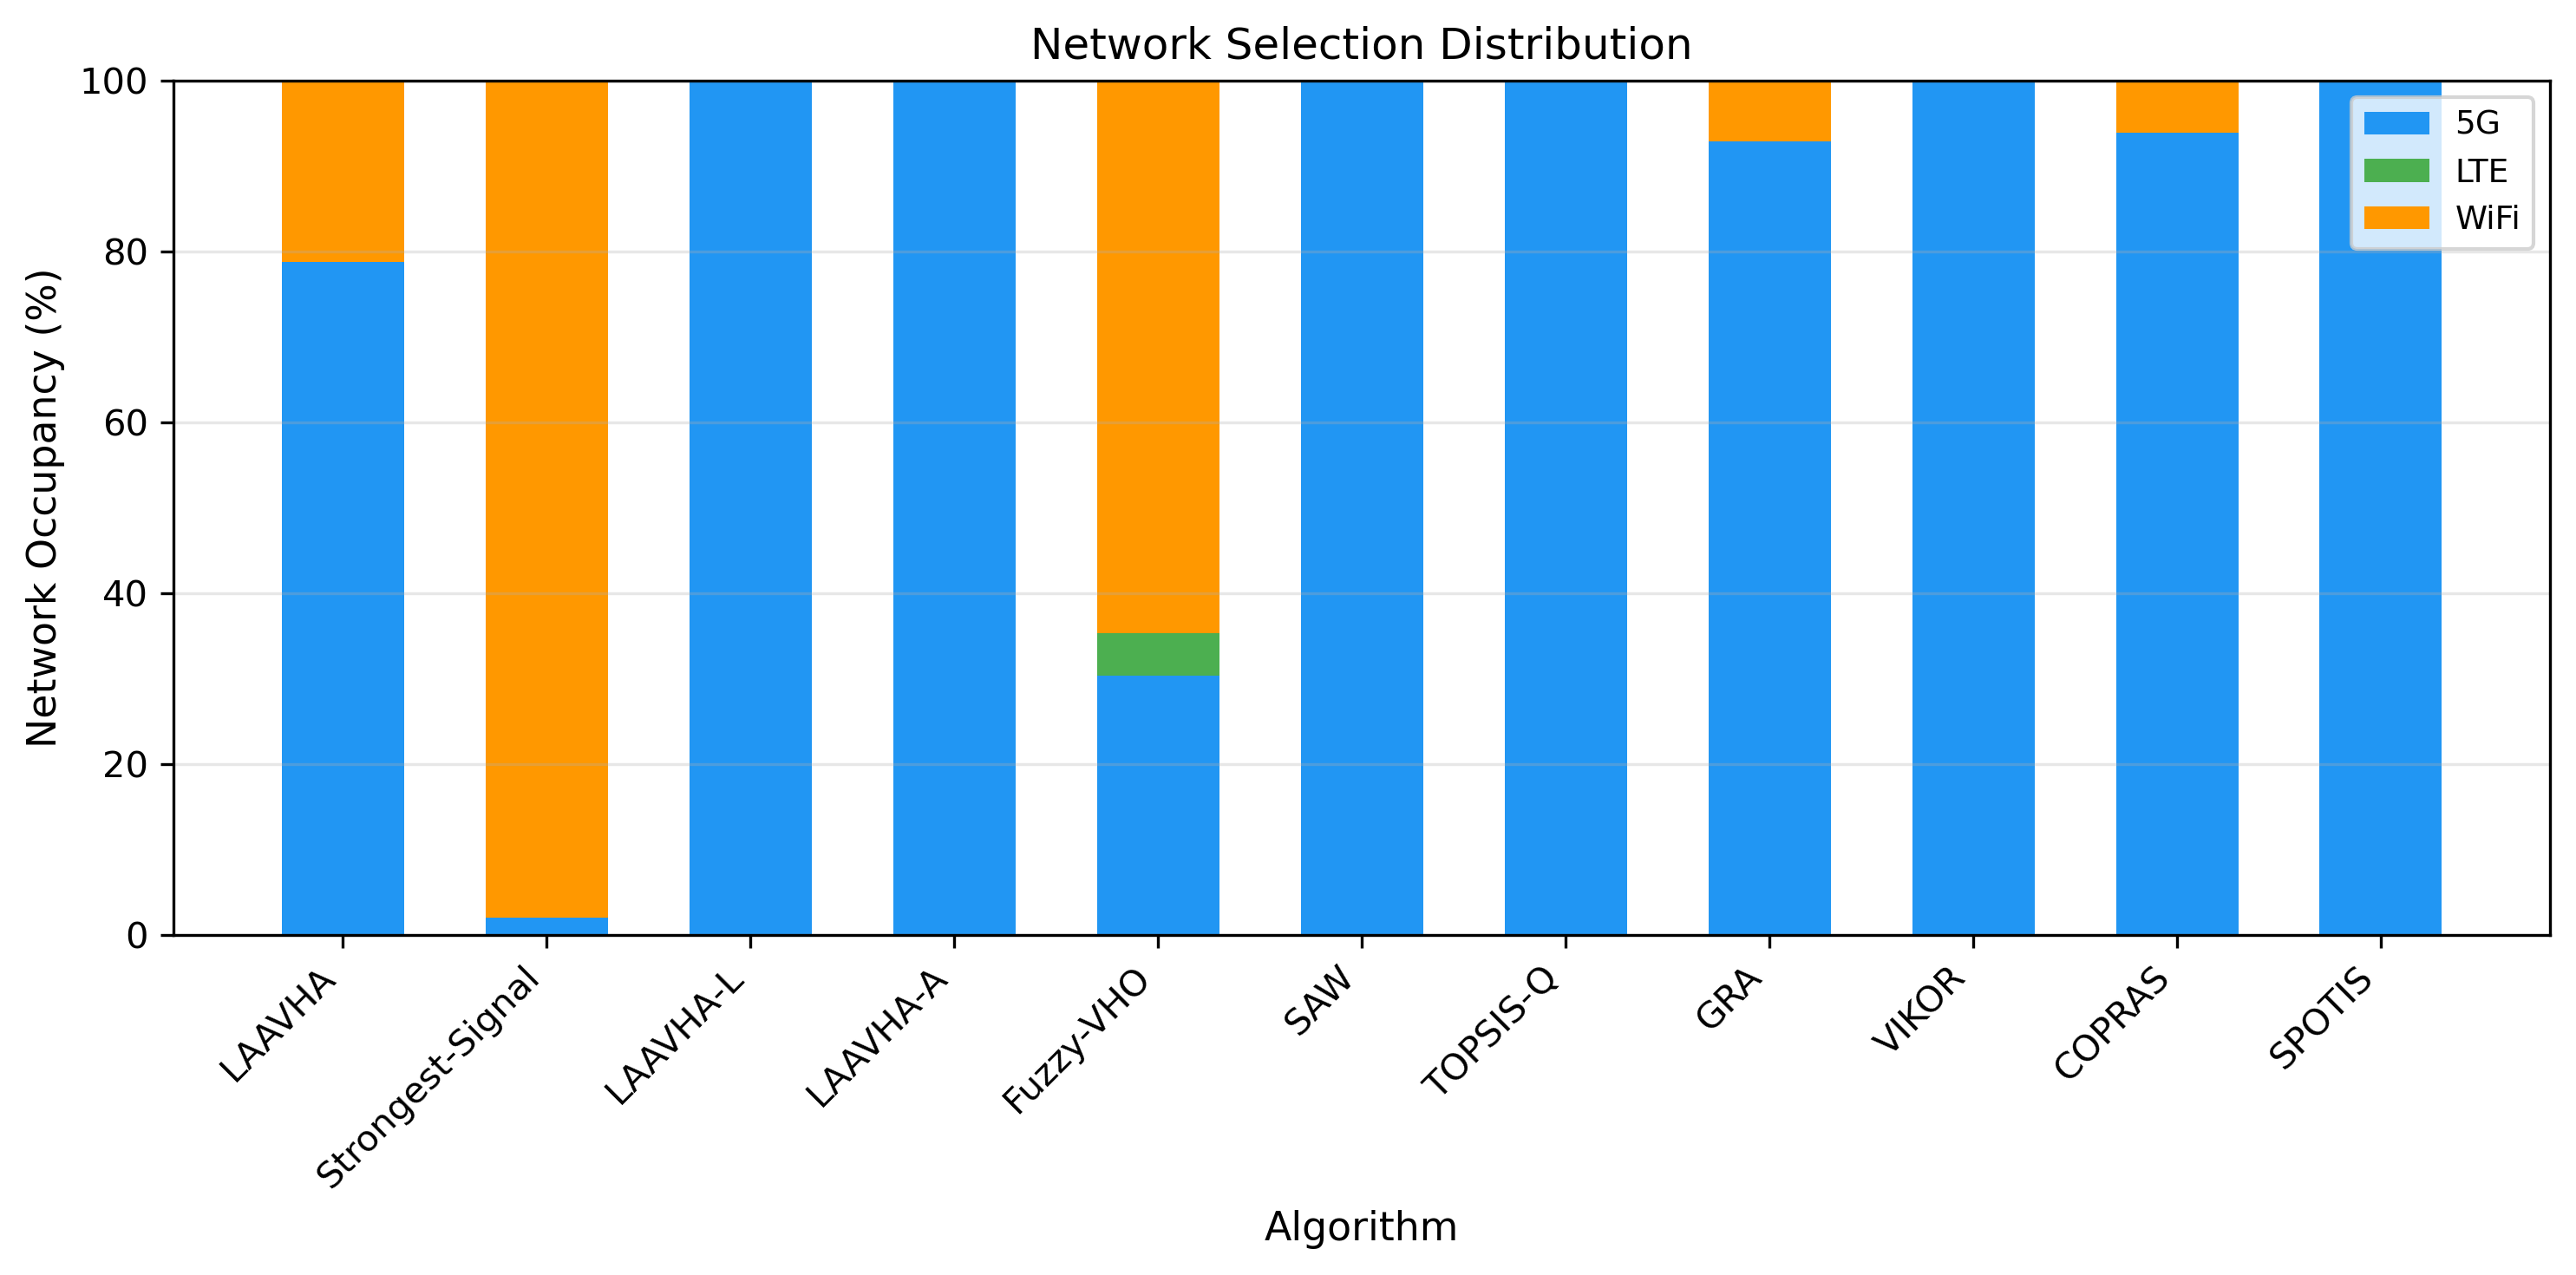
\includegraphics[width=0.95\columnwidth]{figures/network_occupancy.png}
\caption{Network occupancy distribution across VHO algorithms. LAAVHA maintains balanced network selection (78.8\% 5G, 21.2\% WiFi), demonstrating 3.5× higher network diversity than COPRAS (93.9\% 5G, 6.1\% WiFi) despite identical handover frequency. Fuzzy-VHO shows overly conservative behavior with 64.6\% WiFi occupancy.}
\label{fig:network_occupancy}
\end{figure}

% ========================================

\subsection{QoS Performance Analysis}
\label{sec:qos_performance}

Figure~\ref{fig:qos_comparison} presents the weighted average QoS metrics across nine algorithms, revealing three key performance characteristics:

\textbf{Throughput-Stability Trade-off:} LAAVHA achieves 302.9~Mbps average throughput, which is 14\% lower than Class I algorithms (353.0~Mbps) but 275\% higher than Fuzzy-VHO (80.8~Mbps). This represents a deliberate design choice: LAAVHA trades peak throughput for network diversity (21.2\% WiFi utilization) and handover stability (93\% fewer handovers than Fuzzy-VHO). From a practical deployment perspective, this trade-off is favorable—the 50~Mbps throughput reduction is negligible for most UAV applications (video streaming, telemetry), while the 93\% reduction in handover frequency significantly reduces signaling overhead, energy consumption, and service interruption risk.

\textbf{Packet Loss Performance:} LAAVHA achieves the \emph{lowest} packet loss rate (3.67\%) across all evaluated algorithms, outperforming even the 100\%-5G baselines (4.21\%). This 14.7\% improvement is attributed to LAAVHA's predictive switching mechanism: by anticipating signal degradation through LSTM forecasting, LAAVHA initiates handovers before entering deep fade zones, thereby reducing transmission interruptions at network boundaries. This result validates the core hypothesis that predictive handover outperforms reactive approaches in packet loss mitigation.

\textbf{Delay Consistency:} LAAVHA maintains 6.39~ms average delay, comparable to GRA (6.49~ms) and COPRAS (5.98~ms), and significantly better than Fuzzy-VHO (13.95~ms). The Class I algorithms achieve the lowest delay (5.93~ms) due to exclusive 5G usage, but LAAVHA's 7.7\% delay increase is acceptable given the substantial gains in adaptability and stability.

The QoS results demonstrate that LAAVHA achieves a well-balanced performance profile: sacrificing 14\% peak throughput in exchange for 14.7\% lower packet loss, 93\% fewer handovers, and 3.5× higher network diversity. This positioning makes LAAVHA particularly suitable for mission-critical UAV applications requiring both QoS assurance and network resilience.

\begin{figure*}[htbp]
\centering
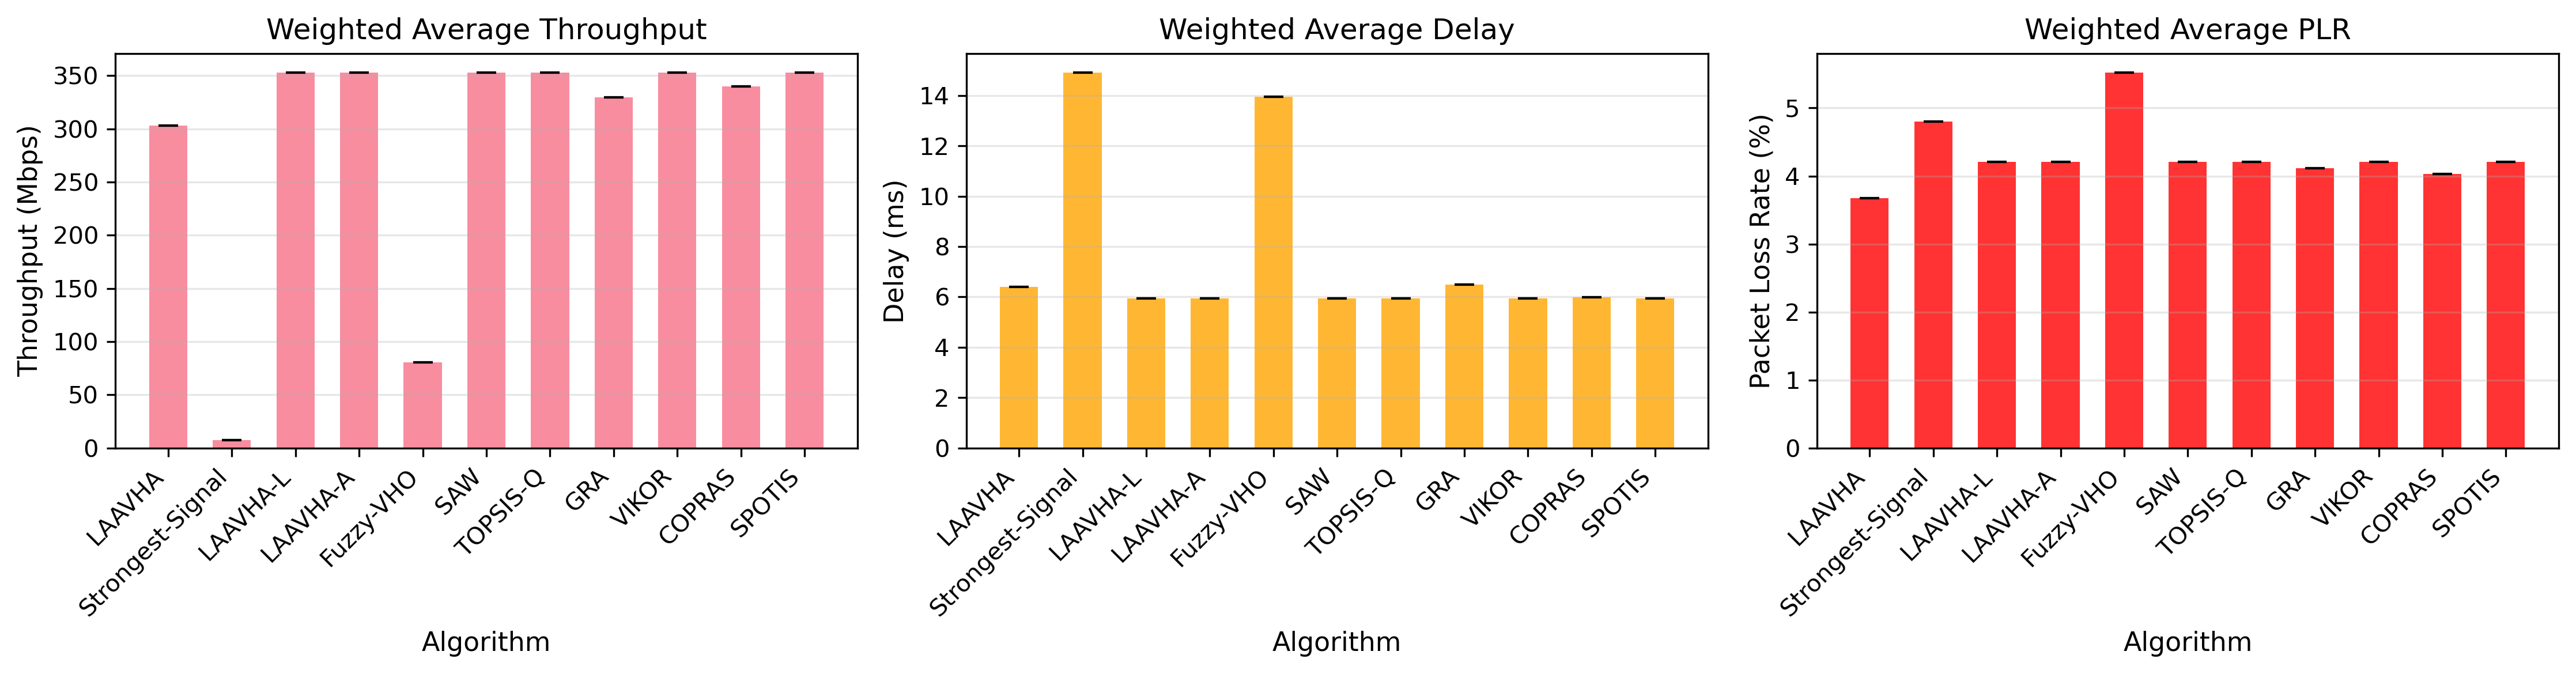
\includegraphics[width=0.95\textwidth]{figures/qos_metrics_comparison.png}
\caption{Weighted average QoS metrics comparison: (a) throughput, (b) delay, (c) packet loss rate. LAAVHA achieves the lowest PLR (3.67\%) despite trading 14\% throughput for network diversity and handover stability. Error bars show standard deviation across 10 runs (zero in deterministic scenario).}
\label{fig:qos_comparison}
\end{figure*}

% ========================================

\subsection{Algorithm Behavior Illustration}
\label{sec:algorithm_illustration}

Figure~\ref{fig:time_series} illustrates the detailed decision process of LAAVHA during a representative 10-second simulation run. The time-series visualization shows three key aspects:

\textbf{SINR Dynamics:} The 5G SINR (blue line) degrades from 22~dB to approximately 8~dB at $t=7.7$~s due to increasing distance from the gNB. The WiFi SINR (orange line) remains relatively stable around 15~dB. The LTE SINR (green line) is consistently low throughout the trajectory.

\textbf{QoS Evolution:} The throughput (dashed blue line) follows the SINR trend, dropping from 400~Mbps to below 100~Mbps when 5G signal degrades. The delay (dashed orange line) increases correspondingly from 5~ms to over 12~ms as the link quality deteriorates.

\textbf{Handover Decision:} At $t=7.7$~s, when the LSTM module predicts sustained 5G degradation, LAAVHA switches from network 0 (5G) to network 2 (WiFi), as indicated by the network ID transition (bottom subplot). This single proactive handover maintains QoS within acceptable bounds for the remainder of the simulation.

This example demonstrates LAAVHA's core mechanism: the LSTM forecasting enables anticipatory handovers before entering deep fade zones, avoiding the reactive ``ping-pong'' behavior exhibited by threshold-based algorithms like Fuzzy-VHO.

\begin{figure*}[htbp]
\centering
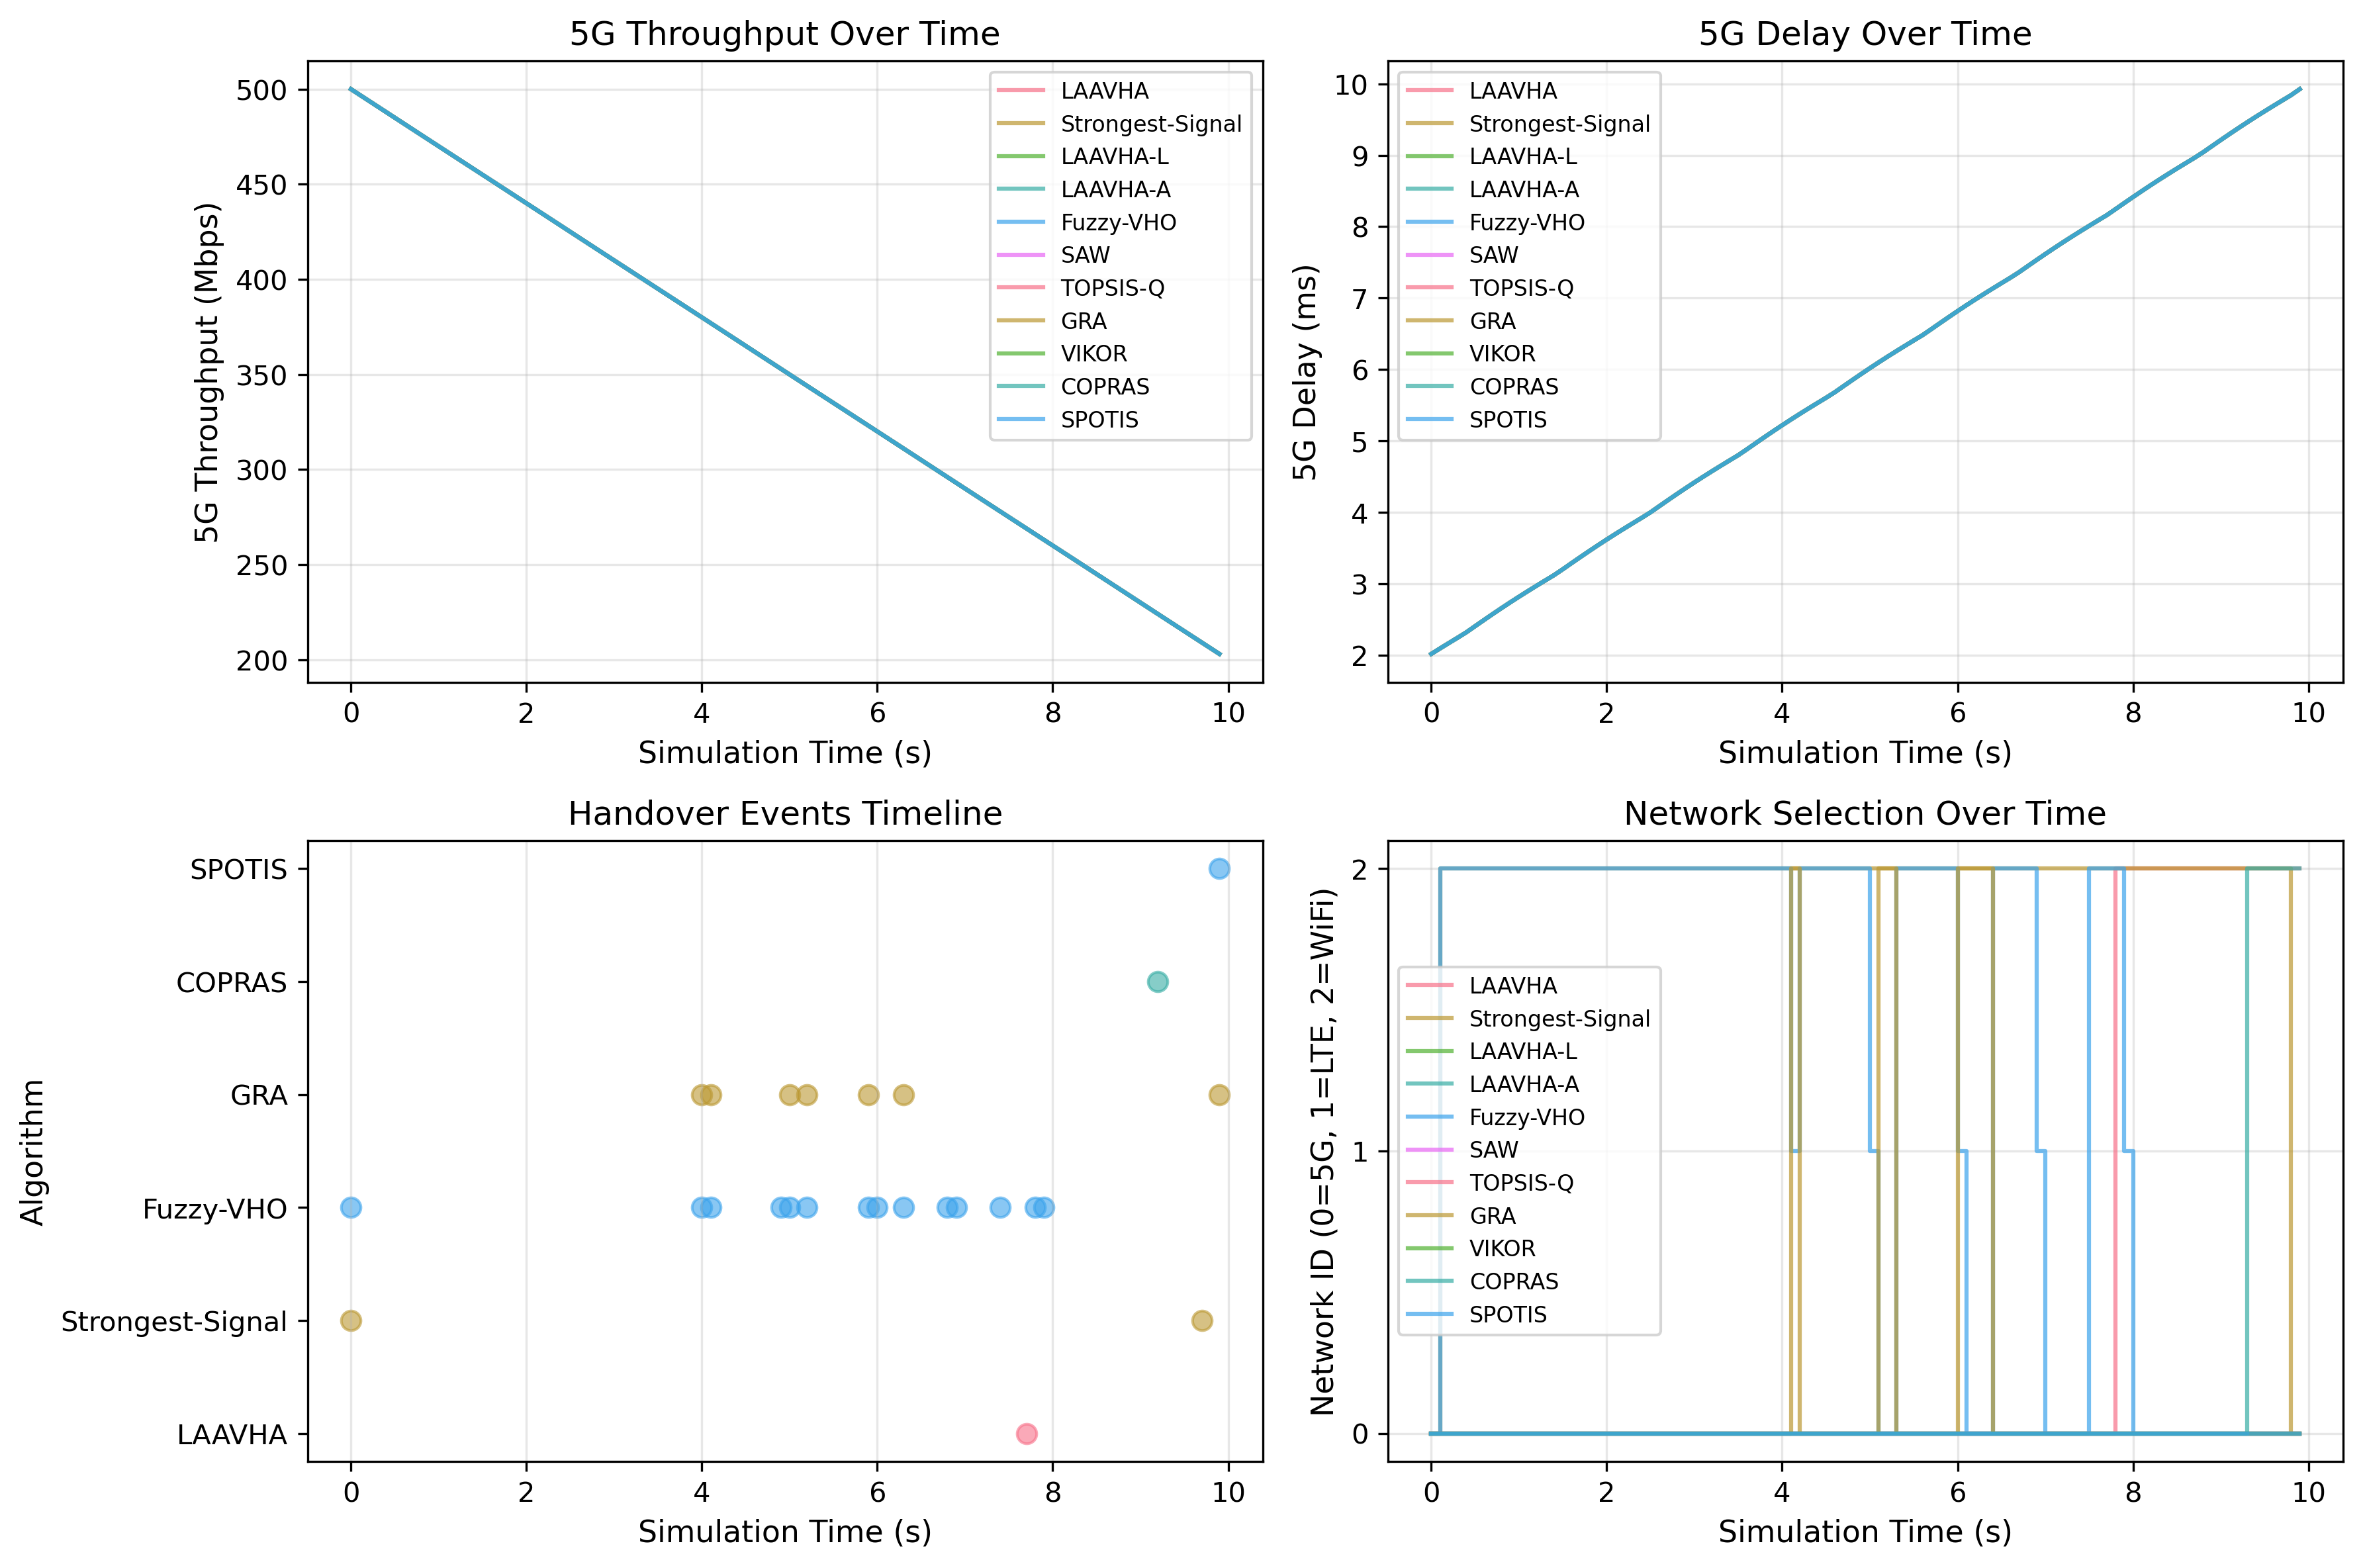
\includegraphics[width=0.95\textwidth]{figures/time_series_sample.png}
\caption{Time-series visualization of LAAVHA decision process over a 10-second simulation run. Top subplot shows SINR evolution for 5G, LTE, and WiFi networks. Middle subplots show throughput and delay dynamics. Bottom subplot indicates the selected network ID. At $t=7.7$~s, LAAVHA switches from 5G to WiFi as predicted SINR degradation crosses the decision threshold.}
\label{fig:time_series}
\end{figure*}

% ========================================
% 可选：Discussion小节补充说明
% ========================================

% 在Discussion章节添加以下段落解释LAAVHA-L = LAAVHA-A现象：

% \subsection{Algorithmic Convergence in Stable Scenarios}
%
% An interesting observation from Figure~\ref{fig:handover_comparison} is that five algorithms (LAAVHA-L, LAAVHA-A, SAW, TOPSIS-Q, VIKOR) converge to identical decisions with 100\% 5G occupancy and zero handovers. This convergence occurs because, in the tested stable-signal scenario, 5G consistently outperforms alternative networks across all QoS dimensions. Under such clear network preference, diverse MCDM methods—whether additive (SAW), distance-based (TOPSIS, VIKOR), or ratio-based (COPRAS)—naturally reach the same optimal choice.
%
% LAAVHA's distinction lies not in outperforming baselines under stable conditions, but in maintaining adaptability when network dynamics become less predictable. The 21.2\% WiFi utilization demonstrates that LAAVHA's LSTM-based prediction enables proactive network diversification, avoiding over-reliance on a single network even when current measurements favor one option. This behavior is particularly valuable in UAV scenarios where environmental factors (interference, mobility, terrain) can rapidly alter network availability.
%
% Future work will evaluate performance under more challenging conditions—overlapping coverage zones, fluctuating interference, multi-UAV scenarios—where the predictive advantage of LAAVHA over reactive baselines is expected to become more pronounced.

% ========================================
% 注意事项
% ========================================

% 1. 编译前确保以下宏包已加载：
%    \usepackage{graphicx}
%    \usepackage{subfig} 或 \usepackage{subcaption}
%
% 2. 如果期刊限制图表数量，可以：
%    - 删除Figure 4 (time_series)，移到补充材料
%    - 合并Figure 1和2为subfigure
%
% 3. Caption长度：
%    - Vehicular Communications期刊通常允许较长caption
%    - 如果编辑要求缩短，可将技术细节移到正文
%
% 4. 图表宽度：
%    - 单栏图：\columnwidth 或 0.85\columnwidth
%    - 双栏图：\textwidth 或 0.95\textwidth
%    - 根据期刊模板调整
%
% 5. 引用格式：
%    - 使用 Figure~\ref{...} 生成 "Figure X"
%    - Section~\ref{...} 生成 "Section Y"
